% !TeX program = xelatex

\documentclass[12pt, a4paper]{report}
\usepackage[top=1in,left=1in,bottom=1.5in,right=1in]{geometry}
\usepackage{hyphenat}
\usepackage{ragged2e}

\newlength\tindent
\setlength{\tindent}{\parindent}
\setlength{\parindent}{0pt}
\renewcommand{\indent}{\hspace*{\tindent}}

\usepackage{fontspec}
\setmainfont[Ligatures=TeX]{Times New Roman}

\usepackage{amsfonts}
\usepackage{amssymb}
\usepackage{amsmath}
\usepackage{amsthm}

\usepackage{bm}
\usepackage{caption}
\usepackage{subcaption}
\usepackage{float}
\usepackage{afterpage}

\usepackage{tikz}

\usepackage{mathtools}
\DeclarePairedDelimiter{\ceil}{\lceil}{\rceil}
\DeclarePairedDelimiter{\floor}{\lfloor}{\rfloor}

\theoremstyle{definition}
\newtheorem{definition}{Definition}

\theoremstyle{definition}
\newtheorem{theorem}{Theorem}

\theoremstyle{remark}
\newtheorem*{remark}{Remark}

\theoremstyle{definition}
\newtheorem*{corollary*}{Corollary}

\theoremstyle{definition}
\newtheorem*{conjecture*}{Conjecture}

\pagenumbering{gobble}

\begin{document}

\setlength{\abovedisplayskip}{0pt}
\setlength{\belowdisplayskip}{0pt}
\setlength{\abovedisplayshortskip}{0pt}
\setlength{\belowdisplayshortskip}{0pt}

{\centering
	\fontsize{14pt}{12pt}
	\textbf{An Attempt to Generalize the Edge Irregularity Strength}\\
	\textbf{of $\bm{m\times n\times l}$ Grid Graphs}
	
	\vspace{9pt}
	
	\begin{tabular}{cc}
		Abyoso Hapsoro Nurhadi$^1$ & Andry Wijaya$^1$\\
		Eunike Setiawan$^1$ & Rabiyatul Adawiyah Haserra$^1$\\
	\end{tabular}
	
	\vspace{8pt}
	
	$^1$Department of Mathematics, University of Indonesia\\
	\{abyoso.hapsoro, andry.wijaya71, ike, rabil.haserra\}@sci.ui.ac.id
\par}

\vspace{5pt}
\makebox[\linewidth]{\rule{\textwidth}{0.1pt}}

\subsubsection*{ABSTRACT}
\indent The edge irregularity strength of a simple graph $G$, denoted as $es(G)$, is defined to be the minimum $k$ such that the graph $G$ has an edge irregular $k$-labeling. The vertex labeling $\phi:V(G)\to\{1,2,...,k\}$ is called a vertex $k$-labeling for G. For any edge $xy$ in $G$, its weight is $w_\phi (xy) = \phi(x) + \phi(y)$. If all the edge weights are distinct, then $\phi$ is called an edge irregular $k$-labeling of G.\\
\indent Consider the cartesian product $P_n\Box P_m\Box P_l$ for $n,m,l\geq2$. The formula for the edge irregularity strength for $n,m\geq2$ and $l=2$ has been established however the authors have yet to establish the cases when $l\geq3$ and posed it as an open problem. In this paper, we attempt to generalize these cases.\\
\textit{Keywords}: Cartesian product, Edge irregularity strength, Grid graph, Vertex labeling

\makebox[\linewidth]{\rule{\textwidth}{0.1pt}}

\subsubsection*{1. Introduction}
\indent A graph is a collection of points and lines connecting some (possibly empty) subset of them. We write a graph $G$ as $G=(V,E)$ where $V=V(G)$ is the non-empty set of vertices of $G$ and $E=E(G)$ is the set of edges of $G$.

\begin{definition}{Simple Graph}
\\\indent A simple graph is an unweighted and undirected graph containing no loops or multiple edges.
\end{definition}

\begin{definition}{Connected Graph}
\\\indent A connected graph is a graph which has a path connecting any point to any other point in the graph.
\end{definition}

\begin{definition}{Vertex Degree}
\\\indent The degree of a vertex $v$ of a graph $G$ is the number of edges that are connected to $v$. We denote the degree of a vertex $v$ as $\rho(v)$.
\end{definition}

\begin{definition}{Maximum Vertex Degree}
\\\indent The maximum vertex degree of a graph $G$ is denoted as $\Delta(G)$. This value can be $0$ if $|E(G)|$ is $0$, i.e. there are no edges in $G$.
\end{definition}

\begin{definition}{Path Graph}
\\\indent A path graph is a graph that can be drawn such that all of its vertices and edges lie on a straight line. The two outermost vertices have degree $1$ and the other $n-2$ vertices have degree $2$. The graph is denoted as $P_n$.
\end{definition}

\newpage

\begin{figure}
	\begin{subfigure}[b]{0.32\textwidth}
	\centering
	\resizebox{\linewidth}{!}{
	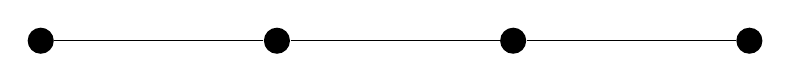
\begin{tikzpicture}[scale=6, every node/.style={circle,fill=black}]
	\tikzset{minimum size=1pt}
	\node (n1) at (0,0)   {};
	\node (n2) at (0.5,0) {};
	\node (n3) at (1,0)   {};
	\node (n4) at (1.5,0) {};
	\foreach \from/\to in {n1/n2, n2/n3, n3/n4}
	\draw (\from) -- (\to);
	\end{tikzpicture}}
	\subcaption{Path Graph $P_4$}
	\end{subfigure}
	\begin{subfigure}[b]{0.32\textwidth}
	\centering
	\resizebox{\linewidth}{!}{
	\begin{tikzpicture}[scale=7, every node/.style={circle,fill=black}]
	\tikzset{minimum size=1pt}
	\node (n1) at (0,0) {};
	\node (n2) at (1,0) {};
	\node (n3) at (0,1) {};
	\node (n4) at (1,1) {};
	\foreach \from/\to in {
		n1/n2, n1/n3,
		n2/n4, n3/n4}
	\draw (\from) -- (\to);
	\end{tikzpicture}}
	\subcaption{Cycle Graph $C_4$}
	\end{subfigure}
	\begin{subfigure}[b]{0.32\textwidth}
	\centering
	\resizebox{\linewidth}{!}{
	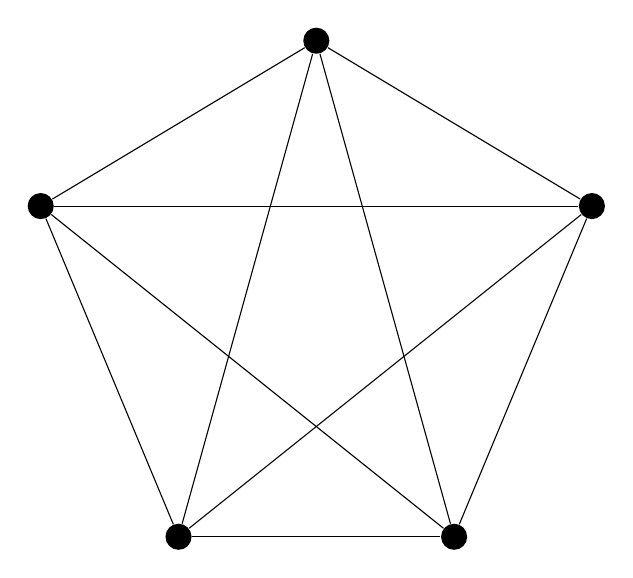
\begin{tikzpicture}[scale=7, every node/.style={circle,fill=black}]
	\tikzset{minimum size=1pt}
	\node (n1) at (0.25,0)  {};
	\node (n2) at (0.75,0)  {};
	\node (n3) at (1,0.6)   {};
	\node (n4) at (0.5,0.9) {};
	\node (n5) at (0,0.6)   {};
	\foreach \from/\to in {
		n1/n2, n1/n3, n1/n4, n1/n5,
		n2/n3, n2/n4, n2/n5,
		n3/n4, n3/n5,
		n4/n5}
	\draw (\from) -- (\to);
	\end{tikzpicture}}
	\subcaption{Complete Graph $K_5$}
	\end{subfigure}
\caption{Some basic graphs}
\end{figure}

Figure 1 shows some examples of simple and connected graphs.

\begin{definition}{Vertex Labeling}
\\\indent A vertex labeling of a graph $G$ is an assignment of integers onto every vertex of $G$.
\end{definition}

\begin{remark}
	The labeling function does not necessarily have to be one-to-one or onto.
\end{remark}

\begin{definition} \textbf{([1])} { Edge Irregularity Strength}
\\\indent Let $G=(V,E)$ be a simple-connected graph. The edge irregular $k$-labeling of a graph $G$ is defined to be the labeling of the vertices of $G$, $\phi:V(G)\to\{1,2,...,k\}$ such that the edge weights $w_\phi (vu) = \phi(v) + \phi(u)$ are distinct for every edge in $G$. The minimum $k$ that satisfies the graph $G$ having an edge irregular $k$-labeling is called the edge irregularity strength of $G$, denoted as $es(G)$.
\end{definition}

\begin{figure}[H]
	\begin{subfigure}[b]{0.48\textwidth}
	\centering
	\resizebox{\linewidth}{!}{
	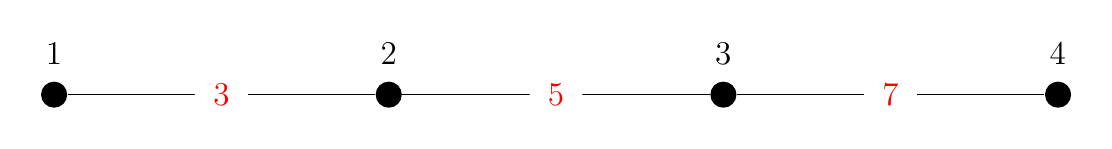
\begin{tikzpicture}[scale=8.5, every node/.style={circle,fill=black}]
	\tikzset{minimum size=1pt}
	\node[label={\large 1}] (n1) at (0,0)   {};
	\node[label={\large 2}] (n2) at (0.5,0) {};
	\node[label={\large 3}] (n3) at (1,0)   {};
	\node[label={\large 4}] (n4) at (1.5,0) {};
	\draw (n1) -- node[label=, red, fill = white] {\large 3} ++ (n2);
	\draw (n2) -- node[label=, red, fill = white] {\large 5} ++ (n3);
	\draw (n3) -- node[label=, red, fill = white] {\large 7} ++ (n4);
	\end{tikzpicture}}
	\subcaption{Edge irregular $4$-labeling of $P_4$}
	\end{subfigure}
	\begin{subfigure}[b]{0.48\textwidth}
	\centering
	\resizebox{\linewidth}{!}{
	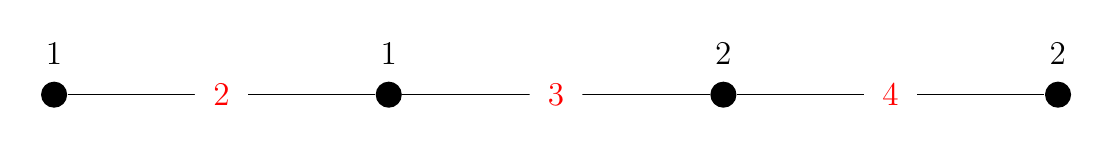
\begin{tikzpicture}[scale=8.5, every node/.style={circle,fill=black}]
	\tikzset{minimum size=1pt}
	\node[label={\large 1}] (n1) at (0,0)   {};
	\node[label={\large 1}] (n2) at (0.5,0) {};
	\node[label={\large 2}] (n3) at (1,0)   {};
	\node[label={\large 2}] (n4) at (1.5,0) {};
	\draw (n1) -- node[label=, red, fill = white] {\large 2} ++ (n2);
	\draw (n2) -- node[label=, red, fill = white] {\large 3} ++ (n3);
	\draw (n3) -- node[label=, red, fill = white] {\large 4} ++ (n4);
	\end{tikzpicture}}
	\subcaption{Edge irregular $2$-labeling of $P_4$}
	\end{subfigure}
	\caption{Two ways to edge irregularly label the vertices of path graph $P_4$}
\end{figure}

\indent We can label the vertices of a graph in more than one way given there are at least two vertices. Figure 2 shows two ways of labeling $P_4$ such that it is an edge irregular labeling. The red text shows the respective edge weights of the graph. A straightforward way to label the vertices so that it is edge irregular is simply to label all the vertices different positive integers which automatically makes it an edge irregular labeling, given in the figure by (a). A better way to label them so that less integers are used is given in the figure by (b). In fact, this is the minimum $k$ that satisfies edge irregularity as labeling every vertex $1$ does not, implying that $es(P_4 )=2$.\\
\indent The following theorem formulates the lower bound for the edge irregularity strength for an arbitrary simple graph $G$.

\begin{theorem} \textbf{([1])}
\\\indent Let $G=(V,E)$ be a simple graph with maximum degree $\Delta=\Delta(G)$. Then,
\begin{equation*}
	es(G) \geq \max \bigg\{ \ceil[\bigg ]{\frac{|E(G)| + 1}{2}}, \Delta(G) \bigg\}
\end{equation*}
\end{theorem}

\newpage

\afterpage{
	\newgeometry{top=1in,left=1in,bottom=1in,right=1in}
	\clearpage
	\restoregeometry
}

\begin{definition}{Graph Cartesian Product}
\\\indent Let there be two graphs, $G_1 = (V_1, E_1)$ and $G_2 = (V_2, E_2)$ where $V_1$ and $V_2$ are disjoint. The cartesian product $G=G_1\Box G_2$, sometimes denoted as $G=G_1\times G_2$, is a graph with $V(G)=V_1\times V_2$ and $u=(u_1,u_2)$ is adjacent with $v=(v_1,v_2)$ whenever [$u_1 = v_1$ and $u_2$ adj $v_2$] or [$u_2 = v_2$ and $u_1$ adj $v_1$].
\end{definition}

\begin{figure}[H]
	\begin{subfigure}[b]{0.32\textwidth}
	\centering
	\resizebox{\linewidth}{!}{
	\begin{tikzpicture}[scale=7, every node/.style={circle}]
	\tikzset{minimum size=1pt}
	\node (n1) at (0,0.1) {};
	\node[fill=black,label=left:$v_1$] (n2) at (0.5,0.1){};
	\node (n3) at (1,0.1) {};
	\node[fill=black,label=left:$u_1$] (n4) at (0.5,0.7) {};
	\node (n5) at (0,0)   {};
	\draw (n2) -- (n4);
	\end{tikzpicture}}
	\subcaption{Path Graph $P_2$}
	\end{subfigure}
	\begin{subfigure}[b]{0.32\textwidth}
	\centering
	\resizebox{\linewidth}{!}{
	\begin{tikzpicture}[scale=6, every node/.style={circle}]
	\tikzset{minimum size=1pt}
	\node (n1) at (0,0)      {};
	\node (n2) at (0.5,0)    {};
	\node (n3) at (1,0)      {};
	\node[fill=black,label=above:$u_2$] (n4) at (0,0.5)  {};
	\node[fill=black,label=above:$v_2$] (n5) at (0.5,0.5){};
	\node[fill=black,label=above:$w_2$] (n6) at (1,0.5)  {};
	\node (n7) at (0,1)    {};
	\node (n8) at (0.5,1)  {};
	\node (n9) at (1,1)    {};
	\node (n10) at (1.2,1) {};
	\foreach \from/\to in {n4/n5, n5/n6}
	\draw (\from) -- (\to);
	\end{tikzpicture}}
	\subcaption{Path Graph $P_3$ \ \ \ \ \ \ }
	\end{subfigure}
	\begin{subfigure}[b]{0.32\textwidth}
	\centering
	\resizebox{\linewidth}{!}{
	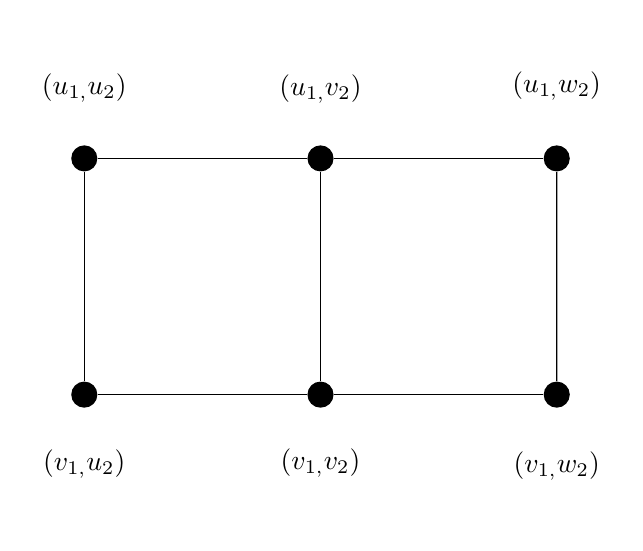
\begin{tikzpicture}[scale=6, every node/.style={circle,fill=black}]
	\tikzset{minimum size=1pt}
	\node[label=below:$(v_{1,}u_2)$] (n1) at (0,0)     {};
	\node[label=below:$(v_{1,}v_2)$] (n2) at (0.5,0)   {};
	\node[label=below:$(v_{1,}w_2)$] (n3) at (1,0)     {};
	\node[label=above:$(u_{1,}u_2)$] (n4) at (0,0.5)   {};
	\node[label=above:$(u_{1,}v_2)$] (n5) at (0.5,0.5) {};
	\node[label=above:$(u_{1,}w_2)$] (n6) at (1,0.5)   {};
	\foreach \from/\to in {
		n1/n2, n1/n4,
		n2/n3, n2/n5,
		n4/n5, n5/n6,
		n3/n6}
	\draw (\from) -- (\to);
	\end{tikzpicture}}
	\subcaption{Cartesian Product $P_2\Box P_3$}
	\end{subfigure}
	\caption{The domino graph $P_2\Box P_3$}
\end{figure}

The cartesian product was introduced in 1950 by Gert Sabidussi along with strong and weak multiplication graph operations [3].

\subsubsection*{2. $\bm{m\times n\times l}$ grid graph}
\indent Consider the cartesian product $P_n\Box P_m\Box P_l$ for $m,n,l\geq2$. When we draw this, we will attain an $m\times n\times l$ grid graph.

\begin{figure}[H]
	\begin{subfigure}[b]{0.48\textwidth}
	\centering
	\resizebox{\linewidth}{!}{
	\begin{tikzpicture}[scale=6, every node/.style={circle,fill=black}]
	\tikzset{minimum size=1pt}
	\node (n1) at (0,0)     {};
	\node (n2) at (1,0)     {};
	\node (n3) at (0.5,0.5) {};
	\node (n4) at (1.5,0.5) {};
	\node (n5) at (0,1)     {};
	\node (n6) at (1,1)     {};
	\node (n7) at (0.5,1.5) {};
	\node (n8) at (1.5,1.5) {};
	\foreach \from/\to in {
		n1/n2, n1/n3, n1/n5,
		n2/n4, n2/n6,
		n3/n4, n3/n7,
		n4/n8,
		n5/n6, n5/n7,
		n6/n8,
		n7/n8}
	\draw (\from) -- (\to);
	\end{tikzpicture}}
	\subcaption{}
	\end{subfigure}
	\begin{subfigure}[b]{0.48\textwidth}
	\centering
	\resizebox{\linewidth}{!}{
	\begin{tikzpicture}[scale=8, every node/.style={circle,fill=black}]
	\tikzset{minimum size=1pt}
	\node (n1) at (0.4,0.4) {};
	\node (n2) at (0.8,0.4) {};
	\node (n3) at (0.4,0.8) {};
	\node (n4) at (0.8,0.8) {};
	\node (n5) at (0,0)     {};
	\node (n6) at (1.2,0)   {};
	\node (n7) at (0,1.2)   {};
	\node (n8) at (1.2,1.2) {};
	\foreach \from/\to in {
		n1/n2, n1/n3, n1/n5,
		n2/n4, n2/n6,
		n3/n4, n3/n7,
		n4/n8,
		n5/n6, n5/n7,
		n6/n8,
		n7/n8}
	\draw (\from) -- (\to);
	\end{tikzpicture}}
	\subcaption{}
	\end{subfigure}
	\caption{(a) Cubical Graph $Q_3=P_2\Box P_2\Box P_2$, (b) The same simpler-drawn graph}
\end{figure}

Figure 4 shows an example of the $m\times n\times l$ grid graph with $m=n=l=2$.

\newpage

\subsubsection*{3. Edge irregularity strength of $\bm{m\times n\times l}$ grid graph}
\indent The following theorem establishes the edge irregularity strength of the $m\times n\times l$ grid graph, i.e. the cartesian product $P_n\Box P_m\Box P_l$ for $n,m\geq 2$ and a fixed $l=2$.

\begin{theorem} \textbf{([5])}
\\\indent Let $G=P_n\Box P_m\Box P_2$ where $m,n\geq2$. Then,
\begin{equation*}
	es(G) = \ceil[\bigg ]{\frac{5mn-2m-2n+1}{2}}
\end{equation*}
\end{theorem}

\vspace{14pt}
The above theorem is achievable using the following labeling function defined by the authors.
\[ \phi_3 (x_i y_j z_r) = \begin{cases} 
	\frac{i-1}{2}(5m-2) + \floor[\big ]{\frac{r}{2}}(m-1) + \ceil[\big ]{\frac{j+r-1}{2}}, & \text{if $i$ is odd} \\
	\frac{i-1}{2}(5m-2) + 4m + r - \floor[\big ]{\frac{j-r+1}{2}} - 2 \floor[\big ]{\frac{j+r-2}{2}} - 3, & \text{if $i$ is even}
\end{cases} \]

where $V(G)=\{(x_i, y_j, z_r): 1\leq i\leq n, 1\leq j\leq m, 1\leq r\leq 2\}$ and $E(G)=\{(x_i, y_j, z_r)(x_{i+1}, y_j, z_r): 1\leq i\leq n - 1, 1\leq j\leq m, 1\leq r\leq l\} \cup \{(x_i, y_j, z_r)(x_i, y_{j+1}, z_r): 1\leq i\leq n, 1\leq j\leq m - 1, 1\leq r\leq l\} \{(x_i, y_j, z_1)(x_i, y_j, z_2): 1\leq i\leq n, 1\leq j\leq m\}$.

\begin{figure}[H]
\centering
\begin{tikzpicture}[scale=8, every node/.style={circle,fill=black}]
\tikzset{minimum size=1pt}
\node[label=below:6] (n1) at (0.4,0.4) {};
\node[label=below:5] (n2) at (0.8,0.4) {};
\node[label=above:1] (n3) at (0.4,0.8) {};
\node[label=above:1] (n4) at (0.8,0.8) {};
\node[label=below:7] (n5) at (0,0)     {};
\node[label=below:5] (n6) at (1.2,0)   {};
\node[label=above:2] (n7) at (0,1.2)   {};
\node[label=above:3] (n8) at (1.2,1.2) {};
\draw (n1) -- node[label=, red, fill = white] {11} ++ (n2);
\draw (n1) -- node[label=, red, fill = white] {7} ++  (n3);
\draw (n1) -- node[label=, red, fill = white] {13} ++ (n5);
\draw (n2) -- node[label=, red, fill = white] {6} ++  (n4);
\draw (n2) -- node[label=, red, fill = white] {10} ++ (n6);
\draw (n3) -- node[label=, red, fill = white] {2} ++  (n4);
\draw (n3) -- node[label=, red, fill = white] {3} ++  (n7);
\draw (n4) -- node[label=, red, fill = white] {4} ++  (n8);
\draw (n5) -- node[label=, red, fill = white] {12} ++ (n6);
\draw (n5) -- node[label=, red, fill = white] {9} ++  (n7);
\draw (n6) -- node[label=, red, fill = white] {8} ++  (n8);
\draw (n7) -- node[label=, red, fill = white] {5} ++  (n8);
\end{tikzpicture}
\caption{Edge Irregular $7$-labeling of $P_2\Box P_2\Box P_2$}
\end{figure}

\indent Using Theorem 2, we find that $es(P_2\Box P_2\Box P_2) = 7$. Figure 5 shows the edge irregular $7$-labeling of $P_2\Box P_2\Box P_2$ achieved using the $\phi_3$ labeling function. The red text shows the respective edge weights of the graph.\\

\indent The same paper by I. Tarawneh, R. Hasni, and A. Ahmad, that established the above theorem posed the following open problem, “Determine the exact value of $es(P_n\Box P_m\Box P_l)$ for $m,n\geq2$ and $l\geq3$."

\newpage
To generalize the cases where $l\geq3$, we need to establish a lower bound for $P_n\Box P_m\Box P_l$ for $m,n,l\geq3$.

\begin{theorem}
\ \\\indent Let $G=P_n\Box P_m\Box P_l$ where $m,n,l\geq 3$. Then,
\begin{equation*}
	es(G)\geq \ceil[\bigg ]{\frac{3lmn-mn-lm-ln+1}{2}}
\end{equation*}
\end{theorem}

\begin{proof}
\ \\\indent Let $m,n,l\geq3$ and $G=P_n\Box P_m\Box P_l$. For each of the graphs $P_n, P_m, P_l$, it is clear that $\Delta(P_n)=\Delta(P_m)=\Delta(P_l)=2$ by Definition 5. The cartesian product operation will cause $\Delta(P_n\Box P_m)=\Delta(P_n) + \Delta(P_m) = 4$ because every degree of a vertex increases by a maximum of 2. This implies that $\Delta(G) = \Delta(P_n) + \Delta(P_m) + \Delta(P_l) = 6$.\\
\indent Counting the bases, we find $l(n(m-1) + m(n-1))$ edges and counting the sides, we find $mn(l-1)$ edges. Hence, $|E(G)| = l(n(m-1) + m(n-1)) + mn(l-1) = 3lmn - mn - lm - ln$.\\
\indent By Theorem 1 we know that,
\begin{equation*}
	es(G) \geq \max \bigg\{ \ceil[\bigg ]{\frac{3lmn - mn - lm - ln + 1}{2}}, 6 \bigg\}
\end{equation*}
\indent We can find the lowermost value for $es(G)$ by considering the case when $m=n=l=3$. Notice that $\ceil[\big ]{\frac{3lmn - mn - lm - ln + 1}{2}}$ will evaluate to 28. This implies that for any $m,n,l\geq3$, $\ceil[\big ]{\frac{3lmn - mn - lm - ln + 1}{2}}$ will always be higher than $6$. Hence,
\begin{equation*}
	es(G)\geq \ceil[\bigg ]{\frac{3lmn-mn-lm-ln+1}{2}}
\end{equation*}
This completes the proof.
\end{proof}

This result is useful, because it helps us know the lower bound of any $P_n\Box P_m\Box P_l$ graph where $m,n,l\geq3$.

\begin{corollary*}
\ \\\indent Let $G=P_n\Box P_m\Box P_3$ where $m,n\geq3$. Then,
\begin{equation*}
	es(G)\geq \ceil[\bigg ]{\frac{8mn-3m-3n+1}{2}}
\end{equation*}
\end{corollary*}

Useful as it is, this result isn't the exact edge irregularity strength of $P_n\Box P_m\Box P_l$ for any $m,n,l\geq3$. Therefore, we propose a conjecture to solve this.

\begin{conjecture*}
\ \\\indent Let $G=P_n\Box P_m\Box P_l$ where $m,n,l\geq 2$. Then,
\begin{equation*}
es(G) = \ceil[\bigg ]{\frac{3lmn-mn-lm-ln+1}{2}}
\end{equation*}
\end{conjecture*}

This simply means that we believe that the edge irregularity strength of the graph $P_n\Box P_m\Box P_l$ where $m,n,l\geq2$ is exactly the lower bound. We have yet to attain the proof to this.\\

In the case where $m,n\geq2$ and $l=2$, our conjecture means that:
\begin{equation*}
	es(G) = \ceil[\bigg ]{\frac{5mn-2m-2n+1}{2}}
\end{equation*}
which is exactly the result of Theorem 2.\\

\newpage

In the case where $m=n=l=3$, our conjecture means that $es(P_3\Box P_3\Box P_3) = 28$. But so far, we have managed an edge irregular $29$-labeling, which is still one off.

\begin{figure}[H]
	\begin{subfigure}[b]{0.48\textwidth}
	\centering{
	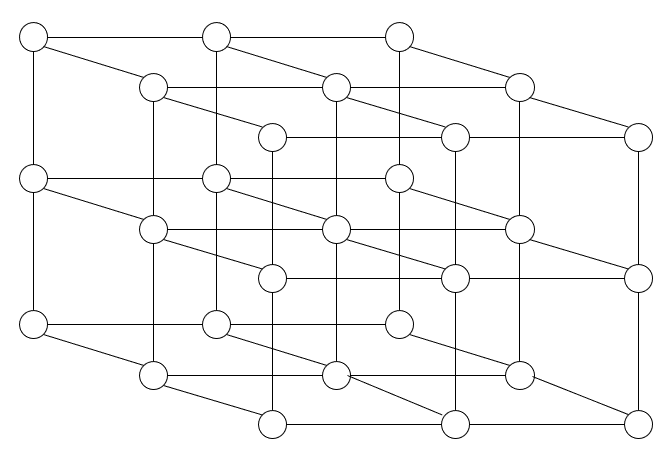
\includegraphics[height=5cm,clip=True]{3x3x3-1.png}
	\par}
	\subcaption{}
	\end{subfigure}
	\begin{subfigure}[b]{0.48\textwidth}
	\centering{
	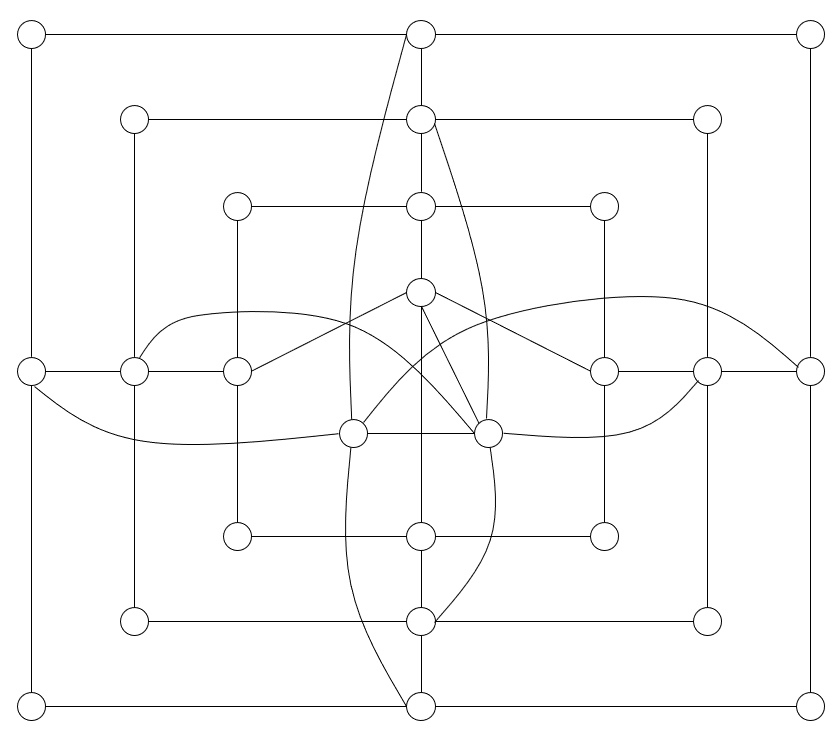
\includegraphics[height=5cm,clip=True]{3x3x3-2.png}
	\par}
	\subcaption{}
	\end{subfigure}
	\caption{(a) Cubical Graph $Q_4=P_3\Box P_3\Box P_3$, (b) The same simpler-drawn graph}
\end{figure}

\begin{figure}[H]
\centering{
	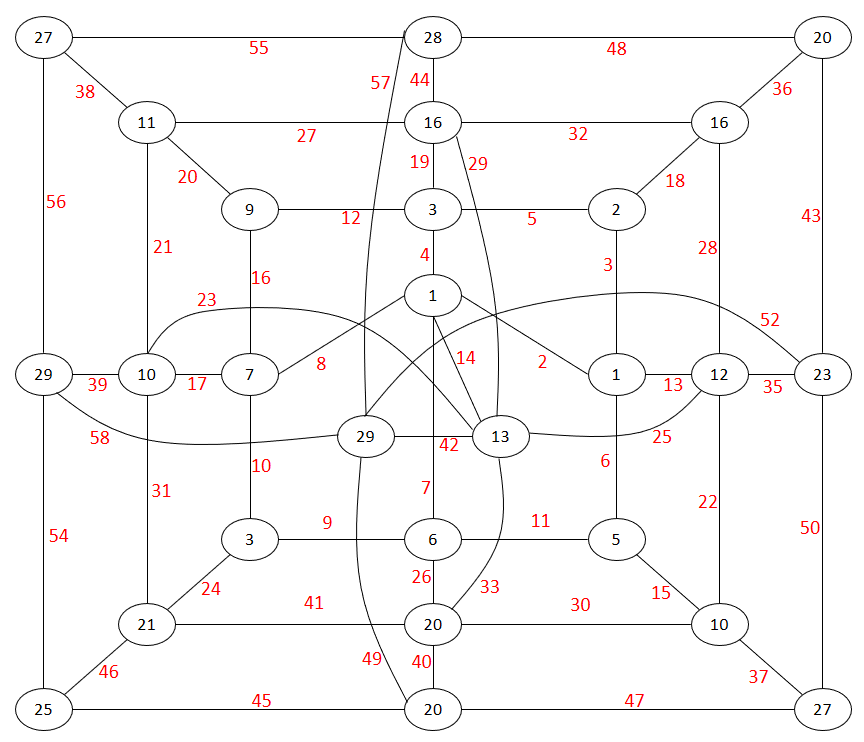
\includegraphics[height=10cm,clip=True]{Labeled3x3x3.png}
\par}
\caption{Edge Irregular $29$-labeling of $P_3\Box P_3\Box P_3$}
\end{figure}

Figure 6 shows the graph $P_3\Box P_3\Box P_3$ and Figure 7 shows the edge irregular 29-labeling of $P_3\Box P_3\Box P_3$ that we have managed. The red text shows the respective edge weights of the graph. Since an edge irregular 29-labeling of $P_3\Box P_3\Box P_3$ is possible and because by Theorem 3, $es(P_3\Box P_3\Box P_3)\geq28$, this implies that $es(P_3\Box P_3\Box P_3)$ is either 28 or 29. We still believe that an edge irregular $28$-labeling of $P_3\Box P_3\Box P_3$ is possible because notice that up to the highest edge weight $58$, the edge weights $34, 51,$ and $53$ are not used in Figure 7.

\newpage

\subsubsection*{4. Conclusion}
\indent In this paper, we discussed the $m\times n\times l$ grid graph, i.e. the cartesian product $P_n\Box P_m\Box P_l$ where $m,n,l\geq2$ and its edge irregularity strength. We managed to obtain the lower bound of $es(P_n\Box P_m\Box P_l)$ for any $m,n,l\geq3$.

\subsubsection*{Acknowledgement}
\indent The authors would like to thank our teacher Dr. Kiki Ariyanti Sugeng, M.Si., Ph.D. for the opportunity to explore this topic as a final project for the Graph Theory course.

\subsubsection*{References}
Ahmad, A., Al-Mushayt, O. and Baca, M. (2014). \textit{On edge irregular strength of graphs}.\\
\indent\indent Appl. Math. Comput. 243, 607-610.\\
Gallian, J. A. (2017). \textit{A Dynamic Survey of Graph Labeling}. The Electronic Journal of\\
\indent\indent Combinatorics, 1-432.\\
Sabidussi, G. (1959). \textit{Graph Multiplication}. Mathematische Zeitschrift, Volume 72, pp 446-\\
\indent\indent 457.\\
Sugeng, K. A., Slamet, S., and Silaban, D. R. (2017). \textit{Teori Graf dan Aplikasinya}.\\
\indent\indent Department of Mathematics University of Indonesia.\\
Tarawneh, I., Hasni, R., and Ahmad, A. (2018). \textit{On the edge irregularity strength of grid}\\
\indent\indent \textit{graphs}. AKCE International Journal of Graphs and Combinatorics.\\
Weisstein, E. W. \textit{Grid Graph}. MathWorld. Accessed 1 January 2019.

\end{document}